

\chapter{Referencial Teórico}
\label{chap:referencial-teorico}

\section{MLP (Perceptron Multicamadas)}

Como é mostrado na Figura \ref{fig:subfigura1}, uma Rede Neural Multicamadas (MLP – \textit{MultiLayer Perceptron})
é formada por um conjunto de neurônios, também conhecidos como
Perceptrons. Uma MLP consiste em uma camada de entrada, juntamente com uma ou mais camadas ocultas.
No processo de treinamento, é empregada uma técnica chamada retropropagação (\textit{backpropagation}), que
ocorre em duas fases distintas: a propagação para frente (\textit{forward}) e a retropropagação propriamente
dita (\textit{backward}), assim como ilustra a Figura \ref{fig:subfigura2}. Durante a propagação para frente, os dados são passados pela rede, camada por camada,
permitindo que as saídas da rede sejam calculadas. Em seguida, durante a fase de retropropagação, os
erros entre as saídas previstas e os valores reais são calculados e propagados de volta através da rede,
ajustando os pesos das conexões para minimizar esses erros. Esse processo iterativo é fundamental para o
treinamento eficaz de uma MLP, permitindo que ela aprenda e se adapte \cite{su12114776}.  

\begin{figure}[h]
    \centering
    \begin{subfigure}{0.40\textwidth}
      \centering
      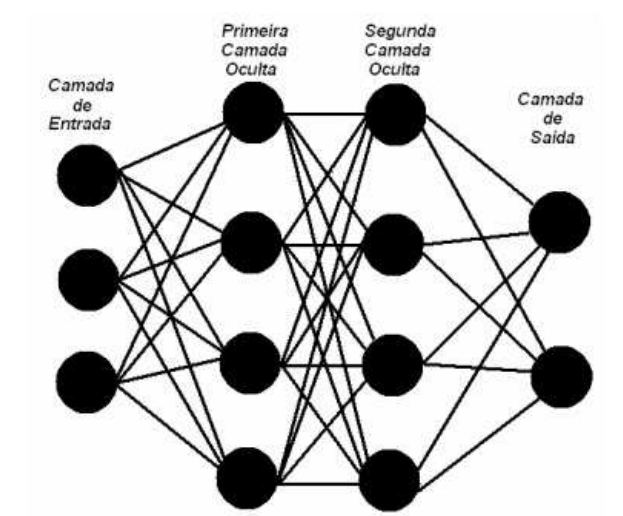
\includegraphics[width=\linewidth]{figuras/MLP/rede_MLP.png}
      \caption{Camadas de uma MLP.}
      \label{fig:subfigura1}
    \end{subfigure}
    \hfill
    \begin{subfigure}{0.45\textwidth}
      \centering
      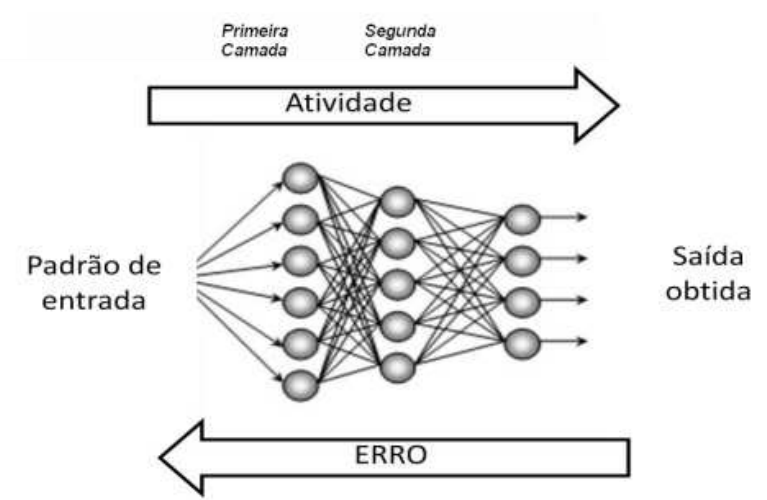
\includegraphics[width=\linewidth]{figuras/MLP/atividade_MLP.png}
      \caption{\textit{Forward} e \textit{backward} em uma rede MLP.}
      \label{fig:subfigura2}
    \end{subfigure}
    \caption{Estrutura e atividade de uma rede MLP, imagem de \cite{su12114776}.}
    \label{fig:subfiguras}
  \end{figure}

%   Neste exemplo, duas figuras estão sendo colocadas lado a lado como subfiguras. O parâmetro {0.45\textwidth} determina a largura de cada subfigura em relação à largura do texto (pode ser ajustado conforme necessário). As sublegendas (\caption) e os rótulos (\label) podem ser personalizados para cada subfigura.
  
%   Para referenciar as subfiguras no texto, você pode usar \ref{} com os rótulos atribuídos às subfiguras. Por exemplo:
%   latex
%   Copy code
%   Como mostrado nas subfiguras \ref{fig:subfigura1} e \ref{fig:subfigura2}, ...
%   Dessa forma, você pode colocar figuras lado a lado como subfiguras em seu documento LaTeX. Certifique-se de compilar seu documento para ver o resultado final.
  
  
  
  
  
  
\section{Naive Bayes}

\section{SVM com kernel RBF}

\section{SVM com kernel Polinomial}

\section{SVM com kernel Linear}
